\chapter[Fundamentação Teórica]{\textbf{F}undamentação \textbf{T}eórica}
%\addcontentsline{toc}{chapter}{Fundamentação Teórica}

\textit{Neste capítulo será apresentado o sistema GSAN e software Asterisk, com a intenção de familiarizar o leitor com as notações que serão amplamente utilizadas no decorrer do trabalho.}


\section{GSAN}
O sistema de código aberto GSAN (Sistema Integrado de Gestão de Serviços de Saneamento) desenvolvido inicialmente pela empresa IPAD (Instituto de Planejamento e Apoio ao Desenvolvimento Tecnológico e Científico) em 2005 por meio do Programa de Modernização do Ministério da Cidades, atualmente mantido e disponibilizado pelo Portal de Software Livre Brasileiro, sendo constantemente melhorado e aperfeiçoado pelos prestadores de serviços e interessados. Propõem-se em atender as principais demandas de gestão de operações comerciais e controle de execução de serviços nas companhias de saneamento do Brasil, que atualmente utilizam o sistema em grande escala, conforme exposto a seguir pela figura \ref{figura:implantacaoSistemaGSAN}:


\begin{figure}[H]
	\centering
	\caption{Implantações do Sistema GSAN}	
	\label{figura:implantacaoSistemaGSAN}
	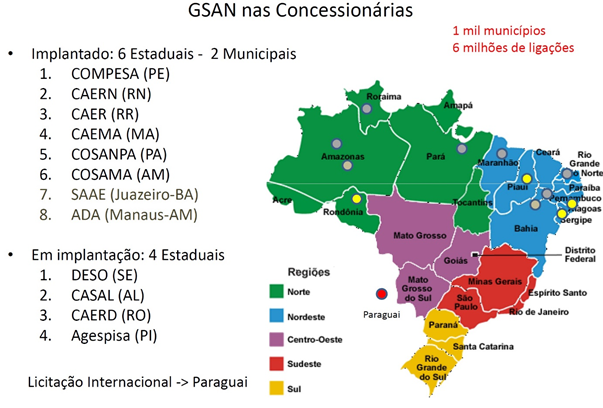
\includegraphics{figuras/implantacaoGSAN.png}
	\legend {\fontsize{10}{12}\selectfont {Fonte: \citeonline{PORTAL:2014}}.}
\end{figure}


Conforme demonstrado acima o sistema está em funcionamento em aproximadamente 1 mil municípios brasileiros, concentrado principalmente na região Nordeste e Norte do Brasil. Atualmente o sistema está preparado para atender companhias de pequeno e médio porte, provendo soluções flexíveis através de parametrizações em tabelas de banco de dados, adequando-se a realidades distintas e tornando-se referência em software para o setor de saneamento básico brasileiro. 

\subsection{GSAN Conceitos}

O sistema em sua concepção foi dividido nos seguintes módulos descritos abaixo:

\begin{itemize}
\item \textbf{Atendimento ao Público}: Responsável principalmente em fornecer acesso rápido as informações dos clientes/imóveis e possibilita o registro dos atendimentos realizados. \\
\item \textbf{Cadastro}: Responsável em permitir a inserção, alteração e exclusão das entidades básicas só sistema. \\
\item \textbf{Micromedição}: Aborda as regras de consistência e análise de leitura e consumo, provendo meios para verificar o comportamento do consumo de água do imóvel. \\
\item \textbf{Faturamento}: Responsável principalmente em realizar o cálculo para precificar o consumo e gerar/emitir as faturas. \\
\item \textbf{Arrecadação}: Disponibiliza meios para efetuar a baixa de débitos dentre outras rotinas dessa natureza. \\
\item \textbf{Segurança}: Possibilita a gestão sobre as permissões de usuários/funcionários. \\
\item \textbf{Cobrança}: Fornece meios de emitir formas de cobranças personalizadas. \\
\item \textbf{Contabilização}: Realiza a contabilidade e possibilita integrações para sistemas externos. \\
\end{itemize}

Alguns dos conceitos de saneamento serão abordados neste trabalho, portanto faz-se necessário conhecer e entender como o sistema GSAN aborda essas questões.
O imóvel no sistema deve possuir relação com os seguintes itens (Tabela \ref{tabela:atributosImovel}):


\begin{table}[H]
	\center
	\footnotesize
	\caption{Principais Atributos do Imóvel}
	\label{tabela:atributosImovel}
	\begin{tabular}{|p{3cm}|p{7cm}|p{2.5cm}|} \hline
		\textbf{Atributo} 	& \textbf{Descrição}						& \textbf{Obrigatório}  \\ \hline
		Localidade 			& Um conjunto populacional					& Sim \\	\hline
		Setor Comercial 	& Conjunto de quadras, semelhante ao bairro & Sim \\ \hline
		Quadra 				& Denominado normalmente de "quarteirão" 	& Sim \\ \hline			
		Lote 				&  Uma subdivisão da Quadra 				& Sim \\ \hline
		Sub-Lote 			&  Uma subdivisão da Lote 					& Sim \\ \hline
	\end{tabular}
	\legend {\fontsize{10}{12}\selectfont {Fonte: Autoria Própria}.}
\end{table}


Tais relacionamentos são necessários para constituir a matrícula do imóvel, que forma um código único e representa a localização exata do imóvel.\\
\textbf{Matrícula:} [ Localidade ].[ Setor Comercial ].[ Quadra ].[ Lote ].[ Sub-Lote ]  \\
\textit{Ex: 001.015.080.0120.001}

O imóvel pode conter uma Ligação seja ela de Água, Poço e Esgoto, após o cliente realizar o cadastro do imóvel e solicitar a ligação, normalmente quando o imóvel obtém uma Ligação de Água ou Poço, é cobrado uma taxa mensal referente ao Esgoto variando em muito dos casos de 80\% a 100\% do valor a ser cobrado pelo consumo de água. Existem as possíveis situações para a Ligação do imóvel:

\begin{itemize}
	\item \textbf{Ligado}: Imóvel está conectado à rede de distribuição de água.
	\item \textbf{Potencial}: Imóvel está localizado fora do alcance da rede de distribuição de água.
	\item \textbf{Factível}: Imóvel está localizado dentro do alcance da rede de distribuição de água, mas que nunca esteve conectado a ela.
	\item \textbf{Cortado}: Imóvel que possui um dispositivo de vedação do fluxo de água no intuito de interromper o abastecimento.
	\item \textbf{Suprimido}: Imóvel que teve o ramal de água retirado para a interrupção definitiva do abastecimento de água.	
\end{itemize}

O relacionamento entre Clientes e Imóveis no sistema pode ocorrer das seguintes formas:

\begin{itemize}
	\item \textbf{USUÁRIO} – Pessoa que reside no imóvel.
	\item \textbf{PROPRIETÁRIO} – Pessoa que possui a propriedade do bem de direito.
	\item \textbf{RESPONSÁVEL} – Pessoa responsável pelo pagamento de débitos do imóvel.	
\end{itemize}

As solicitações realizadas pelos clientes aos atendentes são denominadas Registros de Atendimentos pelo sistema, comumente chamada de RA, para cada tipo de solicitação seja ela Solicitar Ligação, Solicitar Corte, Informar Falta de Água entre outras, o sistema possui tipos de serviços que devem ser realizados para atender a solicitação, a execução destes serviços é representado por uma  entidade denominada Ordem de Serviço, comumente chamada de OS, o sistema permite que seja configurada a criação de OS automáticas para determinadas solicitações, tornando menos burocrático a formalização das reclamações recebidas.



\subsection{GSAN Arquitetura}
	
O Sistema GSAN foi desenvolvido fundamentalmente utilizando a plataforma JEE (\textit{Java Enterprise Edition}), propriedade da \textit{Oracle Corporation}, em sua versão 5, na época a mais recente. Utiliza os principais serviços e tecnologias oferecidos pela plataforma, como por exemplo, \textit{Enterprise Java Beans} (EJB), \textit{Java Message Service} (JMS) API, \textit{Java Server Pages} 2.1, entre outros.
O GSAN possui uma arquitetura que implementa diversos padrões de projeto, visando facilitar a manutenibilidade e manter a organização dos componentes, segue abaixo o diagrama de componentes conforme a figura \ref{figura:arquiteturaDetalhada}:

\begin{figure}[H]
	\centering
	\caption{Arquitetura Detalhada do Sistema GSAN}	
	\label{figura:arquiteturaDetalhada}
	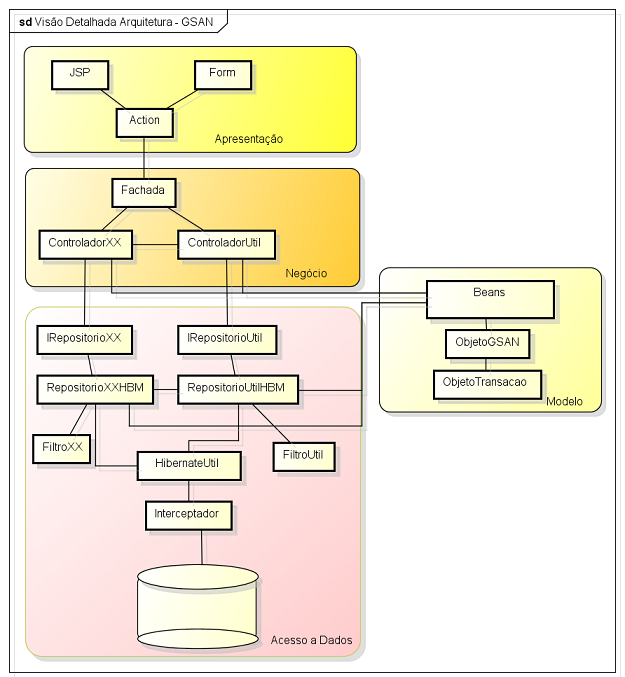
\includegraphics{figuras/gsanArquitetura.png}
	\legend {\fontsize{10}{12}\selectfont {Fonte: Autoria Própria}.}
\end{figure}

	
A camada de apresentação utiliza recurso nativo da plataforma JEE para Web, sendo a JSP (\textit{Java Server Pages}) para construção dos layouts e páginas a serem exibidas, juntamente com o \textit{framework} Apache Struts versão 1.2 atuando como controlador das requisições, além de Javascript e CSS para tratar o comportamento e aparência das páginas.
A fachada é um ponto de comunicação entre as camadas de apresentação e a camada de negócio e implementa o padrão de projeto \textit{Singleton}. A principal função da fachada é centralizar todas as chamadas de métodos da camada de negócio para que outras aplicações ou outras camadas superiores possam utilizar seus serviços.
As Classes de Controladores EJB são responsáveis por garantir toda a regra de negócio do sistema, elas são implementadas utilizando a especificação do \textit{Enterprise Java Beans} (EJB) versão 2.1.
As classes de Repositório são classes da aplicação que utilizam o padrão de projeto \textit{Singleton}, que garante a existência de apenas uma instância desse objeto no sistema, a responsabilidade desta classe consiste em assegurar que todos os métodos de persistência ou serviço de consulta com o banco de dados.
O sistema GSAN foi projetado para ser independente da solução de Banco de Dados utilizada, acoplado ao \textit{framework} Hibernate que trata da persistência Objeto/Relacional (ORM), possibilita o isolamento da camada de Persistência. Fazendo uso de padrões de projetos renomados, tornar o código mais organizado e entendível, facilitando futuras manutenções, a utilização do padrão MVC (\textit{Model View Controller}) como estrutura principal faz com que exista isolamentos entre as camadas de Modelo, Visualização e Controler da aplicação, tornando a organização de pacotes bem estruturada, porém  não houve um bom reaproveitamento de templates, por conta disso foram geradas muitas páginas específicas por funcionalidade e consequentemente muitos arquivos de configuração para o \textit{framework} Struts  que mapeia as requisições via arquivos no formato XML (\textit{eXtensible Markup Language}).
	
	
\subsection{GSAN Configuração}
A configuração do ambiente de desenvolvimento se trata de um passo fundamental para execução deste trabalho prático. Primeiramente será preciso obter a versão do sistema que se encontra disponível no site do Portal do Software Livre, que atualmente disponibiliza o código fonte do sistema GSAN e demais arquivos de configuração do ambiente, no github para a comunidade de desenvolvedores e interessados.  Com o código fonte em mãos será necessário o auxílio de uma IDE (\textit{Integrated Development Environment}) de desenvolvimento para realizar a manutenção e construção dos novos serviços, foi utilizado neste trabalho a IDE Eclipse Juno para realizar esta tarefa, o processo de configuração da IDE pode ser visto descrito nos anexos deste trabalho.
O processo de empacotamento para geração do EAR (\textit{Enterprise Archive}) para disponibilização, utiliza a ferramenta Apache Ant versão 1.6.2, normalmente a versão disponibilizada pela comunidade já possui alguns scripts de build para serem executados, no entanto é preciso configurar os locais adequados para geração do pacote, conforme segue o exemplo abaixo na figura \ref{figura:configuracaoScriptBuild}:


\begin{figure}[H]
	\centering
	\caption{Exemplo de configuração do script build}
	\label{figura:configuracaoScriptBuild}	
	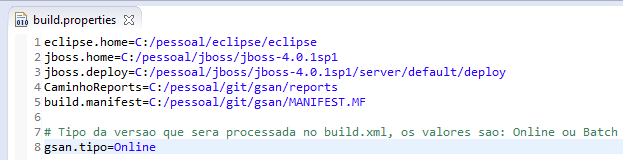
\includegraphics{figuras/build_properties.png}
	\legend {\fontsize{10}{12}\selectfont {Fonte: Autoria Própria}.}
\end{figure}
	
A execução do script pode ser realizada dentro da IDE executando o seguinte procedimento, após localizar o arquivo build.xml dentro na raiz do projeto, ao clicar com o botão esquerdo e selecionar a opção \textit{Run as > Ant Build}, será acionado a execução da instrução \textit{make} padrão do script, para construção do pacote a ser disponibilizado, conforme visto na figura \ref{figura:execucaoScriptBuild}:	
		
\begin{figure}[H]
	\centering
	\caption{Execução do script de build}
	\label{figura:execucaoScriptBuild}
	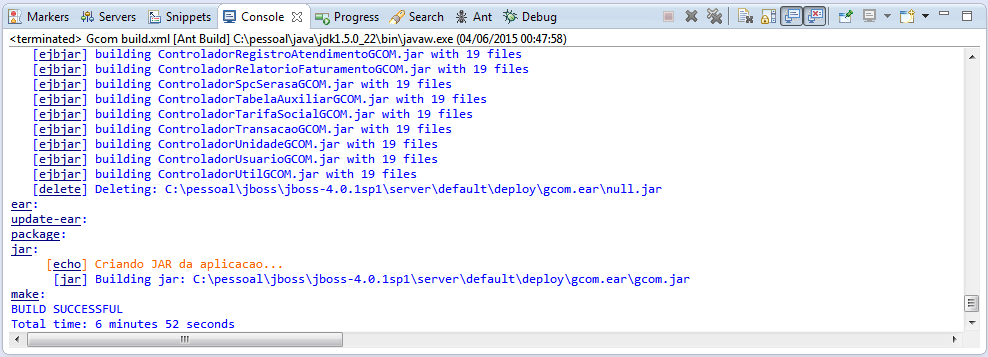
\includegraphics{figuras/build_ant.png}
	\legend {\fontsize{10}{12}\selectfont {Fonte: Autoria Própria}.}
\end{figure}

Para executar a aplicação faz-se necessário a utilização de um servidor de aplicação que implemente as principais interfaces de serviços da plataforma JEE que serão consumidos pela aplicação, neste trabalho foi utilizado o projeto \textit{Open Source Jboss Community} na versão 4.0.1, compatível com as tecnologias utilizadas no GSAN, a configuração deste Servidor de Aplicação Web pode ser consultado nos anexos deste trabalho.
Para executar o sistema GSAN, utilizando o terminal de comando do sistema operacional (\textit{Command Prompt}) basta digitar run e pressionar a tecla Enter será iniciado o servidor de aplicação e executará o sistema GSAN, visto na figura \ref{figura:execucaoSistemaGSAN}:


\begin{figure}[!htb]
	\centering
	\caption{Executando o sistema GSAN}	
	\label{figura:execucaoSistemaGSAN}
	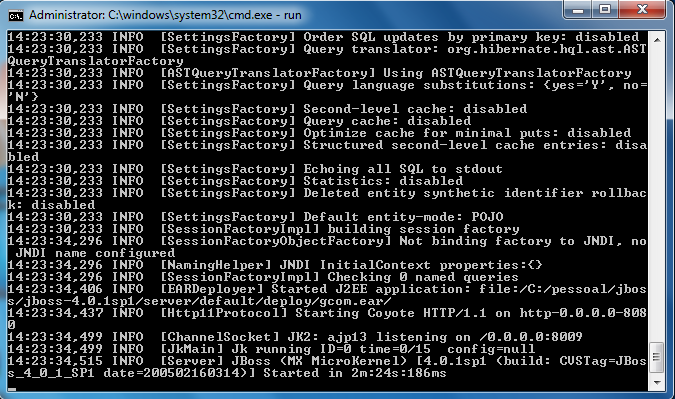
\includegraphics{figuras/executando_jboss.png}	
	\legend {\fontsize{10}{12}\selectfont {Fonte: Autoria Própria}.}
\end{figure}


A solução adotada para banco de dados neste trabalho será o PostgreSQL na versão 9.3.4 e PgAdmin versão 1.18.1 como SGBD (Sistema de Gerenciamento de Banco de Dados), no próprio site existe o guia de instalação para desenvolvedores tornando esse passo bem intuitivo.

Na versão do sistema GSAN disponibilizada para a comunidade, existe um diretório chamado \textbf{\textit{migrations}} que contém os scripts de banco de dados necessários para criação das tabelas principais que o sistema exige para funcionar corretamente, e também disponibiliza todas instruções necessárias para a configuração dos datasources comercial e gerencial que serão utilizados no sistema GSAN.
Para acessar o sistema em execução, basta digitar o seguinte endereço no navegador http://127.0.0.1:8080/gsan, caso tudo ocorra bem deverá ser apresentada a página conforme visto na figura \ref{figura:acessoPaginaInicial} abaixo:

\begin{figure}[!htb]
	\centering
	\caption{Acessando página inicial do Sistema}
	\label{figura:acessoPaginaInicial}	
	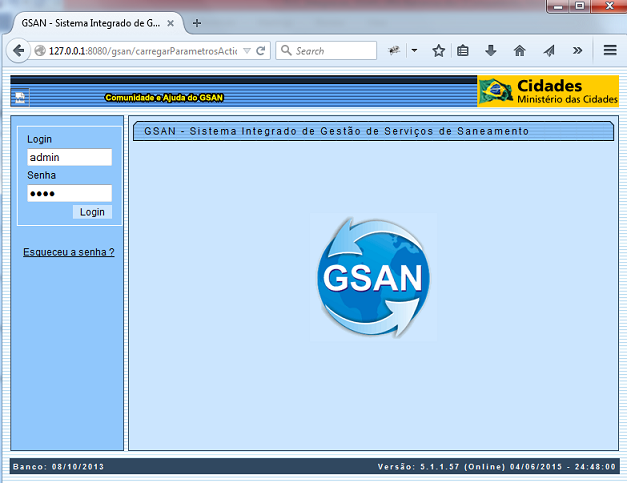
\includegraphics{figuras/gsan_online.png}	
	\legend {\fontsize{10}{12}\selectfont {Fonte: Autoria Própria}.}
\end{figure}


A credencial de acesso criada por padrão é: \\
\textbf{Login}: admin \\
\textbf{Senha}: gcom \\
Após inserir a credencial de acesso acima teremos acesso as todas as funcionalidades dos módulos do sistema GSAN.

